\documentclass[a4paper, 11pt]{article}
%Paquetes%%%%%%%%%%%%%%%%%%%%%%%%%%%%%%%%%%%%%%%%%%%%%%%%%%%%%%%%%%%%%%%%%%%
\usepackage[utf8]{inputenc}
\usepackage[T1]{fontenc}
\usepackage[spanish,es-tabla]{babel}
\usepackage{everypage}
\usepackage{graphicx}
\usepackage{tikz}
\usepackage{color}
\usepackage[left=3cm, right=2.75cm, top=4.5cm, bottom=4cm]{geometry}
\usepackage{fancyhdr}
\usepackage{float}
\pagestyle{empty}
\usepackage{tikzpagenodes}
\usetikzlibrary{calc}
\usepackage{hyperref}
\usepackage{amsmath}
\usepackage{amssymb}
\usepackage{listings}
\usepackage{xcolor}
\usepackage{enumitem}
\usepackage{longtable}
\usepackage{array}

\definecolor{codegray}{rgb}{0.95,0.95,0.95}

\lstset{
  inputencoding=utf8,
  extendedchars=true,
  literate={á}{{\'a}}1 {é}{{\'e}}1 {í}{{\'i}}1 {ó}{{\'o}}1 {ú}{{\'u}}1
           {Á}{{\'A}}1 {É}{{\'E}}1 {Í}{{\'I}}1 {Ó}{{\'O}}1 {Ú}{{\'U}}1
           {ñ}{{\~n}}1 {Ñ}{{\~N}}1,
  backgroundcolor=\color{codegray},
  basicstyle=\ttfamily\small,
  frame=single,
  breaklines=true,
  captionpos=b,
  showstringspaces=false,
  keywordstyle=\color{blue},
  commentstyle=\color{gray},
  stringstyle=\color{red},
  numbers=left,
  numberstyle=\tiny\color{gray},
  stepnumber=1,
  numbersep=8pt,
  xleftmargin=2em,
  framexleftmargin=1.5em
}

\usepackage[user,abspage]{zref}
\renewcommand{\baselinestretch}{1.35}

\hypersetup{%
colorlinks=true, linkcolor=blue, urlcolor=blue,linkbordercolor=blue, urlbordercolor=blue, pdfborderstyle={/S/U/W 1}
}
\makeatletter
\Hy@AtBeginDocument{%
  \def\@pdfborder{0 0 1}%
  \def\@pdfborderstyle{/S/U/W 1}%
}
\makeatother
\definecolor{rojo_oscuro}{rgb}{.85,.45,.45}
\definecolor{verde_oscuro}{rgb}{0,.5,.2}
\AddEverypageHook{%
\tikz[remember picture,overlay]{%
  \ifnum\value{page}>1%
    \filldraw[fill=rojo_oscuro, thick,  draw=verde_oscuro] (1,-1.6) rectangle (16,-1.3);
    \filldraw[fill=rojo_oscuro, thick, draw=verde_oscuro] (1,-1.6-22.8) rectangle (16,-1.3-22.8);
        \node[anchor=east] at (16,-25) {\normalfont\textcolor{black}{{\footnotesize DCCO - ESPE}}};
        \node[anchor=west] at (1,-25) {\normalfont\textcolor{black}{{\footnotesize \thepage}}};
        \node at (1.8,0) {
\includegraphics[width=2.5cm]{DCCO.png}};
  \else
    \filldraw[fill=rojo_oscuro, thick, draw=verde_oscuro] (-0.3,0) rectangle (0.3,-26);
    \filldraw[fill=rojo_oscuro, thick,  draw=verde_oscuro] (1,-1.6) rectangle (16,-1.3);
    \filldraw[fill=rojo_oscuro, thick, draw=verde_oscuro] (1,-1.6-21.8) rectangle (16,-1.3-21.8);
    \node[anchor=east] at (16,-24) {\textit{{\Large Informe del taller de planificación ágil}}};
    \node[anchor=east] at (16,-25) {\textit{{\Large Ing. Jenny Ruiz}}};
    \node[anchor=east] at (16,-25.8) {\textit{{\Large Departamento de Ciencias de la Computación - ESPE}}};
    \node[anchor=east] at (16,-10) {\textbf{{\Huge Análisis y}}};
    \node[anchor=east] at (16,-11) {\textbf{{\Huge Diseño de Software}}};
    \node[anchor=east] at (16,-14.3) {\textbf{{\huge Autores}}};
    \node[anchor=east] at (16,-15.3) {\textit{{\Large Laínez Suárez Ricardo Andrés}}};
    \node[anchor=east] at (16,-16.3) {\textit{{\Large Padilla Triviño Marco Adrian}}};
    \node[anchor=east] at (16,-17.3) {\textit{{\Large Andino Martínez Nelson David}}};
    \node[anchor=east] at (16,-18.3) {\textit{{\Large NRC: 36838}}};
    \node[anchor=east] at (16,-20.6) {\textbf{{\Huge Planificación del proyecto}}};
    \node[anchor=east] at (16,-21.6) {\textbf{{\Huge Bocatto con Jira y Confluence}}};
    \node at (4.2,0.) {
\includegraphics[width=6cm]{Logo.png}};
    \node at (14,0.) {
\includegraphics[width=2.5cm]{DCCO.png}};
  \fi}
  }
%%%%%%%%%%%%%%%%%%%%%%%%%%%%%%%%%%%%%%%%%%%%%%%%%%%%%%%%%%%%%%%%%%%%%%%%%%%
\begin{document}
\zlabel{iniciodedocumento}
\textbf{}
\newpage
\thispagestyle{empty}

\tableofcontents
\newpage

\section{Introducción}

El Grupo 5 de Análisis y Diseño de Software trabaja sobre el sistema de gestión de pedidos del restaurante Bocatto Valley. Con la Especificación de Requisitos (ERS), la matriz IREB y los ocho casos de uso de nivel 0 ya definidos, el siguiente paso fue organizar el trabajo con un marco ágil. Para eso se armó el product backlog en la plantilla entregada por la docente, se repartió el trabajo en sprints cortos y se llevó todo a Jira con la plantilla Scrum.

Cada requisito funcional quedó además documentado en Confluence con su pantalla propuesta (mockup), los datos que maneja y sus reglas de negocio. El repositorio de GitHub se reorganizó con la estructura pedida y el espacio P.A.R.A. de Notion se enlazó con Jira, Confluence y GitHub. Este informe describe ese proceso y deja los enlaces a cada herramienta.

\section{Objetivos}

\subsection{Objetivo general}

Planificar el desarrollo del sistema de pedidos Bocatto con Scrum, registrando el backlog, los sprints y las tareas en Jira y documentando cada requisito funcional en Confluence.

\subsection{Objetivos específicos}

\begin{itemize}
  \item Redactar las historias de usuario de los ocho requisitos funcionales en la plantilla de backlog, con prioridad, notas y responsable.
  \item Dividir las historias en sprints cortos y desglosarlas en tareas con responsable y horas estimadas.
  \item Configurar el proyecto 36838\_G5 en Jira con épicas, historias, subtareas y sprints que coincidan con el backlog.
  \item Documentar en Confluence las vistas, pantallas y el modelo de datos de cada requisito.
  \item Integrar Jira, Confluence y GitHub con el espacio P.A.R.A. del proyecto en Notion.
\end{itemize}

\section{Marco teórico}

\textbf{Scrum.} Es un marco de trabajo ágil en el que el equipo entrega el producto en ciclos cortos llamados sprints. Al inicio de cada sprint se eligen elementos del product backlog y al final se revisa lo terminado \cite{scrumguide}.

\textbf{Product backlog.} Es la lista ordenada de todo lo que necesita el producto. En este proyecto cada elemento es una historia de usuario asociada a un requisito funcional de la ERS.

\textbf{Historia de usuario.} Describe una necesidad desde el punto de vista de quien usa el sistema con la forma \textit{como} (rol), \textit{necesito} (acción), \textit{así podré} (beneficio).

\textbf{Jira.} Herramienta de Atlassian para gestionar proyectos ágiles. Con la plantilla Scrum ofrece backlog, sprints, tablero y una vista de cronograma \cite{jira}.

\textbf{Confluence.} Wiki colaborativa de Atlassian que se integra con Jira. Aquí se usó para la documentación técnica de cada requisito \cite{confluence}.

\section{Desarrollo}

\subsection{Product backlog}

El backlog se completó en la plantilla \texttt{G5\_Backlog\_PlantillaV1.xlsx}. Tiene una fila por requisito funcional, con el tema, la historia de usuario, las notas o criterios, la prioridad y el estado. Los requisitos que sostienen el flujo principal del pedido (acceso, registro por los tres canales, cocina y caja) tienen prioridad alta. La consulta de estado y la administración quedaron en prioridad media. La Tabla \ref{tab:backlog} resume el backlog y la Tabla \ref{tab:hu} muestra cada historia de usuario.

{\small
\begin{longtable}{|p{1.2cm}|p{3.3cm}|p{2.7cm}|p{1.5cm}|p{2.4cm}|p{1.1cm}|}
\caption{Resumen del product backlog del sistema Bocatto.}\label{tab:backlog}\\
\hline
\textbf{ID} & \textbf{Tema} & \textbf{Rol} & \textbf{Prioridad} & \textbf{Encargado} & \textbf{Horas} \\ \hline
\endfirsthead
\hline
\textbf{ID} & \textbf{Tema} & \textbf{Rol} & \textbf{Prioridad} & \textbf{Encargado} & \textbf{Horas} \\ \hline
\endhead
RF001 & Autenticar en el sistema & Personal del restaurante & Alta & Marco Padilla & 5 \\ \hline
RF002 & Tomar pedido en mesa & Mesero & Alta & Marco Padilla & 6 \\ \hline
RF003 & Tomar pedido telefónico & Operador de llamadas & Alta & Ricardo Laínez & 5 \\ \hline
RF004 & Realizar pedido por QR & Cliente & Alta & Marco Padilla & 6 \\ \hline
RF005 & Gestionar preparación del pedido & Cocinero & Alta & Ricardo Laínez & 5 \\ \hline
RF006 & Cobrar pedido en la caja & Cajero & Alta & Nelson Andino & 5 \\ \hline
RF007 & Consultar estado de pedido & Cliente & Media & Nelson Andino & 4 \\ \hline
RF008 & Administrar configuración del sistema & Administrador & Media & Ricardo Laínez & 9 \\ \hline
\end{longtable}
}

{\small
\begin{longtable}{|p{1.2cm}|p{12.5cm}|}
\caption{Historias de usuario del backlog.}\label{tab:hu}\\
\hline
\textbf{ID} & \textbf{Historia de usuario} \\ \hline
\endfirsthead
\hline
\textbf{ID} & \textbf{Historia de usuario} \\ \hline
\endhead
RF001 & Como personal del restaurante, necesito ingresar al sistema con mi usuario y contraseña, así podré acceder solo a las funciones permitidas para mi rol. \\ \hline
RF002 & Como mesero, necesito registrar el pedido de una mesa numerada con productos, cantidades y observaciones, así podré enviar el pedido a cocina sin errores de anotación. \\ \hline
RF003 & Como operador de llamadas, necesito registrar pedidos por llamada con productos, cantidades, observaciones y datos del cliente, así podré que el pedido llegue a cocina igual que un pedido en mesa. \\ \hline
RF004 & Como cliente, necesito escanear el QR de mi mesa y elegir productos del menú digital, así podré hacer mi pedido desde el celular sin esperar al mesero. \\ \hline
RF005 & Como cocinero, necesito ver los pedidos pendientes y actualizar su estado, así podré que el personal y el cliente sepan en qué va cada pedido. \\ \hline
RF006 & Como cajero, necesito buscar el pedido por número de mesa y registrar el método de pago, así podré cobrar el total correcto y habilitar el pedido para la entrega. \\ \hline
RF007 & Como cliente, necesito consultar el estado de mi pedido desde el QR de la mesa, así podré saber cuándo está listo sin preguntar al mesero. \\ \hline
RF008 & Como administrador, necesito gestionar el menú digital, los QR de las mesas, las promociones y consultar reportes básicos, así podré que los pedidos se hagan con información actualizada. \\ \hline
\end{longtable}
}

\subsection{Planificación de los sprints}

Se definieron cuatro sprints cortos, de uno o dos días, entre el 5 y el 9 de noviembre de 2026. El Sprint 0 deja listo el acceso y la configuración que usan los demás módulos. Luego se avanza por el recorrido del pedido: primero el registro en mesa y por QR, después el canal telefónico junto con la cocina, y al final el cobro y la consulta del estado. Cada sprint se representa en Jira como una épica que agrupa sus dos historias (Tabla \ref{tab:sprints}).

{\small
\begin{longtable}{|p{1.6cm}|p{2.6cm}|p{4.3cm}|p{2.6cm}|p{2cm}|}
\caption{Sprints del proyecto y épica de Jira asociada.}\label{tab:sprints}\\
\hline
\textbf{Sprint} & \textbf{Fecha} & \textbf{Objetivo} & \textbf{Requisitos} & \textbf{Épica} \\ \hline
\endfirsthead
Sprint 0 & 5 y 6 de noviembre & Acceso al sistema y configuración base & RF001, RF008 & SCRUM-39 \\ \hline
Sprint 1 & 7 de noviembre & Registro de pedidos en mesa y por QR & RF002, RF004 & SCRUM-40 \\ \hline
Sprint 2 & 8 de noviembre & Pedido telefónico y preparación en cocina & RF003, RF005 & SCRUM-41 \\ \hline
Sprint 3 & 9 de noviembre & Cobro en caja y estado del pedido & RF006, RF007 & SCRUM-42 \\ \hline
\end{longtable}
}

En la hoja de sprints de la plantilla cada historia se desglosó en tareas con el código \texttt{REQ00X-N}, un responsable y su estimado en horas. La Tabla \ref{tab:tareas} muestra todas las tareas.

{\small
\begin{longtable}{|p{1.9cm}|p{7.6cm}|p{2.6cm}|p{1.3cm}|}
\caption{Tareas por sprint con responsable y estimado.}\label{tab:tareas}\\
\hline
\textbf{ID} & \textbf{Tarea} & \textbf{Asignado} & \textbf{Estimado} \\ \hline
\endfirsthead
\hline
\textbf{ID} & \textbf{Tarea} & \textbf{Asignado} & \textbf{Estimado} \\ \hline
\endhead
\multicolumn{4}{|l|}{\textbf{Sprint 0}: Acceso al sistema y configuración base} \\ \hline
REQ001-1 & Diseñar la pantalla de inicio de sesión. & Marco Padilla & 1 h \\ \hline
REQ001-2 & Implementar la validación de usuario y contraseña contra la base de datos. & Marco Padilla & 2 h \\ \hline
REQ001-3 & Asignar permisos y menú de funciones según el rol del usuario. & Ricardo Laínez & 2 h \\ \hline
REQ008-1 & Desarrollar la gestión del menú digital (productos, precios y disponibilidad). & Ricardo Laínez & 3 h \\ \hline
REQ008-2 & Implementar la asignación y generación de códigos QR por mesa. & Marco Padilla & 2 h \\ \hline
REQ008-3 & Desarrollar el registro de promociones vigentes. & Nelson Andino & 2 h \\ \hline
REQ008-4 & Construir la consulta de reportes básicos del negocio. & Ricardo Laínez & 2 h \\ \hline
\multicolumn{4}{|l|}{\textbf{Sprint 1}: Registro de pedidos en mesa y por QR} \\ \hline
REQ002-1 & Diseñar la pantalla de toma de pedido con selección de mesa. & Marco Padilla & 1 h \\ \hline
REQ002-2 & Implementar el registro de productos, cantidades y observaciones. & Marco Padilla & 2 h \\ \hline
REQ002-3 & Validar que el pedido tenga al menos un producto y generar su identificador. & Nelson Andino & 1 h \\ \hline
REQ002-4 & Enviar el pedido en estado pendiente a la pantalla de cocina. & Ricardo Laínez & 2 h \\ \hline
REQ004-1 & Diseñar el menú digital para celular que se abre desde el QR. & Marco Padilla & 2 h \\ \hline
REQ004-2 & Implementar la identificación de la mesa a partir del código QR. & Marco Padilla & 2 h \\ \hline
REQ004-3 & Registrar el pedido del cliente en estado pendiente y enviarlo a cocina. & Ricardo Laínez & 2 h \\ \hline
\multicolumn{4}{|l|}{\textbf{Sprint 2}: Pedido telefónico y preparación en cocina} \\ \hline
REQ003-1 & Diseñar el formulario de pedido telefónico. & Ricardo Laínez & 1 h \\ \hline
REQ003-2 & Registrar los datos del cliente y de entrega o retiro. & Marco Padilla & 2 h \\ \hline
REQ003-3 & Validar y guardar el pedido en estado pendiente y notificar a cocina. & Ricardo Laínez & 2 h \\ \hline
REQ005-1 & Diseñar la pantalla de cocina con la lista de pedidos pendientes. & Ricardo Laínez & 1 h \\ \hline
REQ005-2 & Implementar el cambio de estado en secuencia válida. & Marco Padilla & 2 h \\ \hline
REQ005-3 & Reflejar el estado actualizado para el personal y el cliente. & Nelson Andino & 2 h \\ \hline
\multicolumn{4}{|l|}{\textbf{Sprint 3}: Cobro en caja y estado del pedido} \\ \hline
REQ006-1 & Diseñar la pantalla de caja con búsqueda por número de mesa. & Nelson Andino & 1 h \\ \hline
REQ006-2 & Mostrar el detalle del pedido y calcular el total a pagar. & Marco Padilla & 2 h \\ \hline
REQ006-3 & Registrar el método de pago y marcar el pedido como pagado. & Nelson Andino & 2 h \\ \hline
REQ007-1 & Diseñar la vista de estado del pedido para el cliente. & Nelson Andino & 1 h \\ \hline
REQ007-2 & Consultar el pedido de la mesa a partir del QR. & Marco Padilla & 1 h \\ \hline
REQ007-3 & Mostrar el estado actual en tiempo real. & Nelson Andino & 2 h \\ \hline

\end{longtable}
}

\subsection{Distribución del trabajo}

El trabajo se repartió de forma equilibrada entre los tres integrantes. Cada uno es encargado de al menos dos historias y además apoya con tareas en historias de otros, como se ve en la Tabla \ref{tab:dist}.

\begin{table}[H]
\centering
\small
\begin{tabular}{|l|c|c|c|c|}
\hline
\textbf{Integrante} & \textbf{Historias a cargo} & \textbf{Tareas} & \textbf{Horas} & \textbf{Porcentaje} \\ \hline
Marco Padilla & 3 & 11 & 19 h & 42\% \\ \hline
Ricardo Laínez & 3 & 8 & 15 h & 33\% \\ \hline
Nelson Andino & 2 & 7 & 11 h & 24\% \\ \hline
\textbf{Total} & 8 & 26 & 45 h & 100\% \\ \hline
\end{tabular}
\caption{Distribución de historias, tareas y horas por integrante.}
\label{tab:dist}
\end{table}

\subsection{Configuración del proyecto en Jira}

Se creó el sitio \texttt{36838-g5.atlassian.net} con Jira Free y el proyecto \textbf{36838\_G5} con la plantilla Scrum. Se invitó a los otros dos integrantes con sus correos institucionales. La estructura del proyecto replica el backlog:

\begin{itemize}
  \item \textbf{Épicas:} una por sprint (SCRUM-39 a SCRUM-42).
  \item \textbf{Historias:} una por requisito. El nombre empieza con el código del requisito y el caso de uso (por ejemplo, \textit{RF002 Tomar pedido en mesa}). La descripción incluye la historia de usuario, el caso de uso, las notas, el encargado, el sprint y la lista de tareas.
  \item \textbf{Subtareas:} las tareas de la plantilla, cada una con su responsable y sus horas como puntos de historia.
  \item \textbf{Sprints:} Sprint 0, 1 y 2 cerrados. El Sprint 3 está activo hasta la presentación del taller.
\end{itemize}

{\small
\begin{longtable}{|p{4.6cm}|p{1.9cm}|p{2.6cm}|p{1.5cm}|p{2.6cm}|}
\caption{Historias registradas en Jira con sus subtareas.}\label{tab:jira}\\
\hline
\textbf{Historia} & \textbf{Clave} & \textbf{Subtareas (SCRUM)} & \textbf{Puntos} & \textbf{Encargado} \\ \hline
\endfirsthead
RF001 Autenticar en el sistema & SCRUM-5 & 6 a 8 & 5 & Marco Padilla \\ \hline
RF002 Tomar pedido en mesa & SCRUM-14 & 15 a 18 & 6 & Marco Padilla \\ \hline
RF003 Tomar pedido telefónico & SCRUM-23 & 24 a 26 & 5 & Ricardo Laínez \\ \hline
RF004 Realizar pedido por QR & SCRUM-19 & 20 a 22 & 6 & Marco Padilla \\ \hline
RF005 Gestionar preparación del pedido & SCRUM-27 & 28 a 30 & 5 & Ricardo Laínez \\ \hline
RF006 Cobrar pedido en la caja & SCRUM-31 & 32 a 34 & 5 & Nelson Andino \\ \hline
RF007 Consultar estado de pedido & SCRUM-35 & 36 a 38 & 4 & Nelson Andino \\ \hline
RF008 Administrar configuración del sistema & SCRUM-9 & 10 a 13 & 9 & Ricardo Laínez \\ \hline
\end{longtable}
}

La vista de cronograma de Jira (Figura \ref{fig:jira_crono}) muestra las cuatro épicas en orden con sus historias. La Figura \ref{fig:jira_hist} muestra el detalle de una historia con su descripción y sus subtareas asignadas.

\begin{figure}[H]
  \centering
  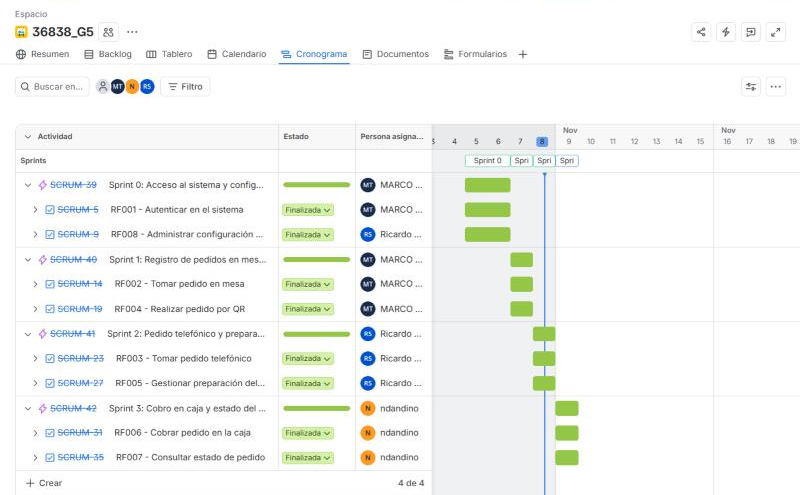
\includegraphics[width=\textwidth]{jira_cronograma.png}
  \caption{Vista de cronograma del proyecto 36838\_G5 en Jira con las épicas de cada sprint.}
  \label{fig:jira_crono}
\end{figure}

\begin{figure}[H]
  \centering
  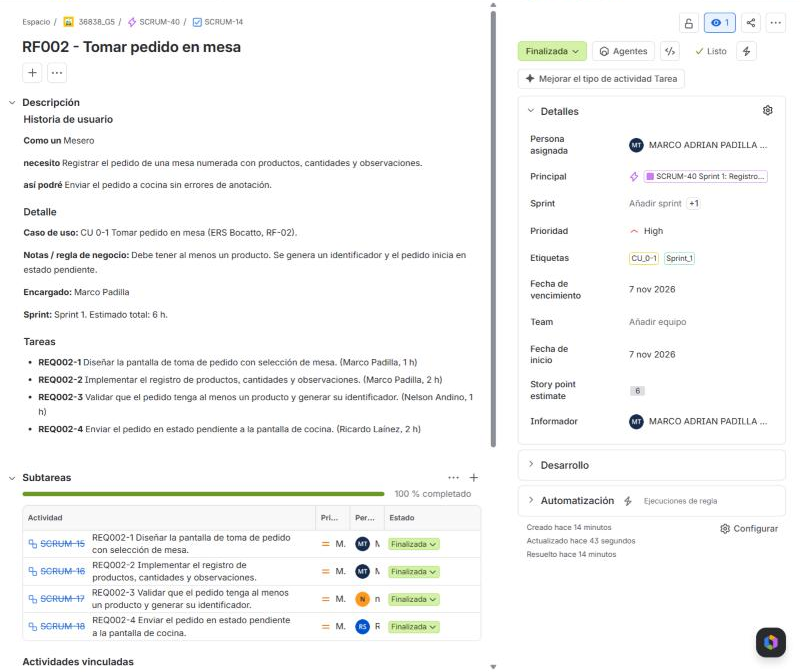
\includegraphics[width=\textwidth]{jira_historia.png}
  \caption{Historia SCRUM-14 (RF002 Tomar pedido en mesa) con su descripción y subtareas en Jira.}
  \label{fig:jira_hist}
\end{figure}

\subsection{Documentación en Confluence}

En el espacio 36838\_G5 de Confluence se creó la página \textit{Maquetado del sistema Bocatto por requisito}, con una subpágina para cada requisito funcional y una para el modelo de datos. Cada subpágina contiene:

\begin{itemize}
  \item La historia de usuario y una tabla con el actor, el caso de uso, la prioridad, el sprint y el encargado.
  \item El enlace a la historia correspondiente en Jira. Desde Jira también se puede abrir la página de Confluence.
  \item El mockup de la pantalla, los elementos que la componen y los datos que usa.
  \item Las reglas de negocio que salen de la ERS.
\end{itemize}

\begin{figure}[H]
  \centering
  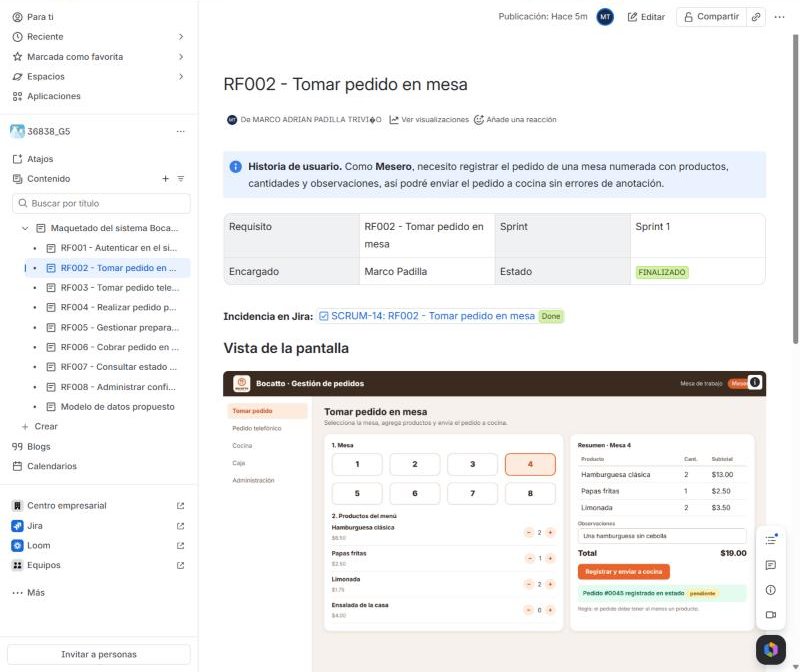
\includegraphics[width=0.9\textwidth]{confluence_rf002.png}
  \caption{Página de Confluence del requisito RF002 con la historia de usuario, el enlace a Jira y el mockup.}
  \label{fig:conf}
\end{figure}

Los mockups usan la paleta de colores del logo de Bocatto. Los productos y precios que aparecen son datos de ejemplo. La Figura \ref{fig:mock} muestra la pantalla del mesero para registrar un pedido en mesa.

\begin{figure}[H]
  \centering
  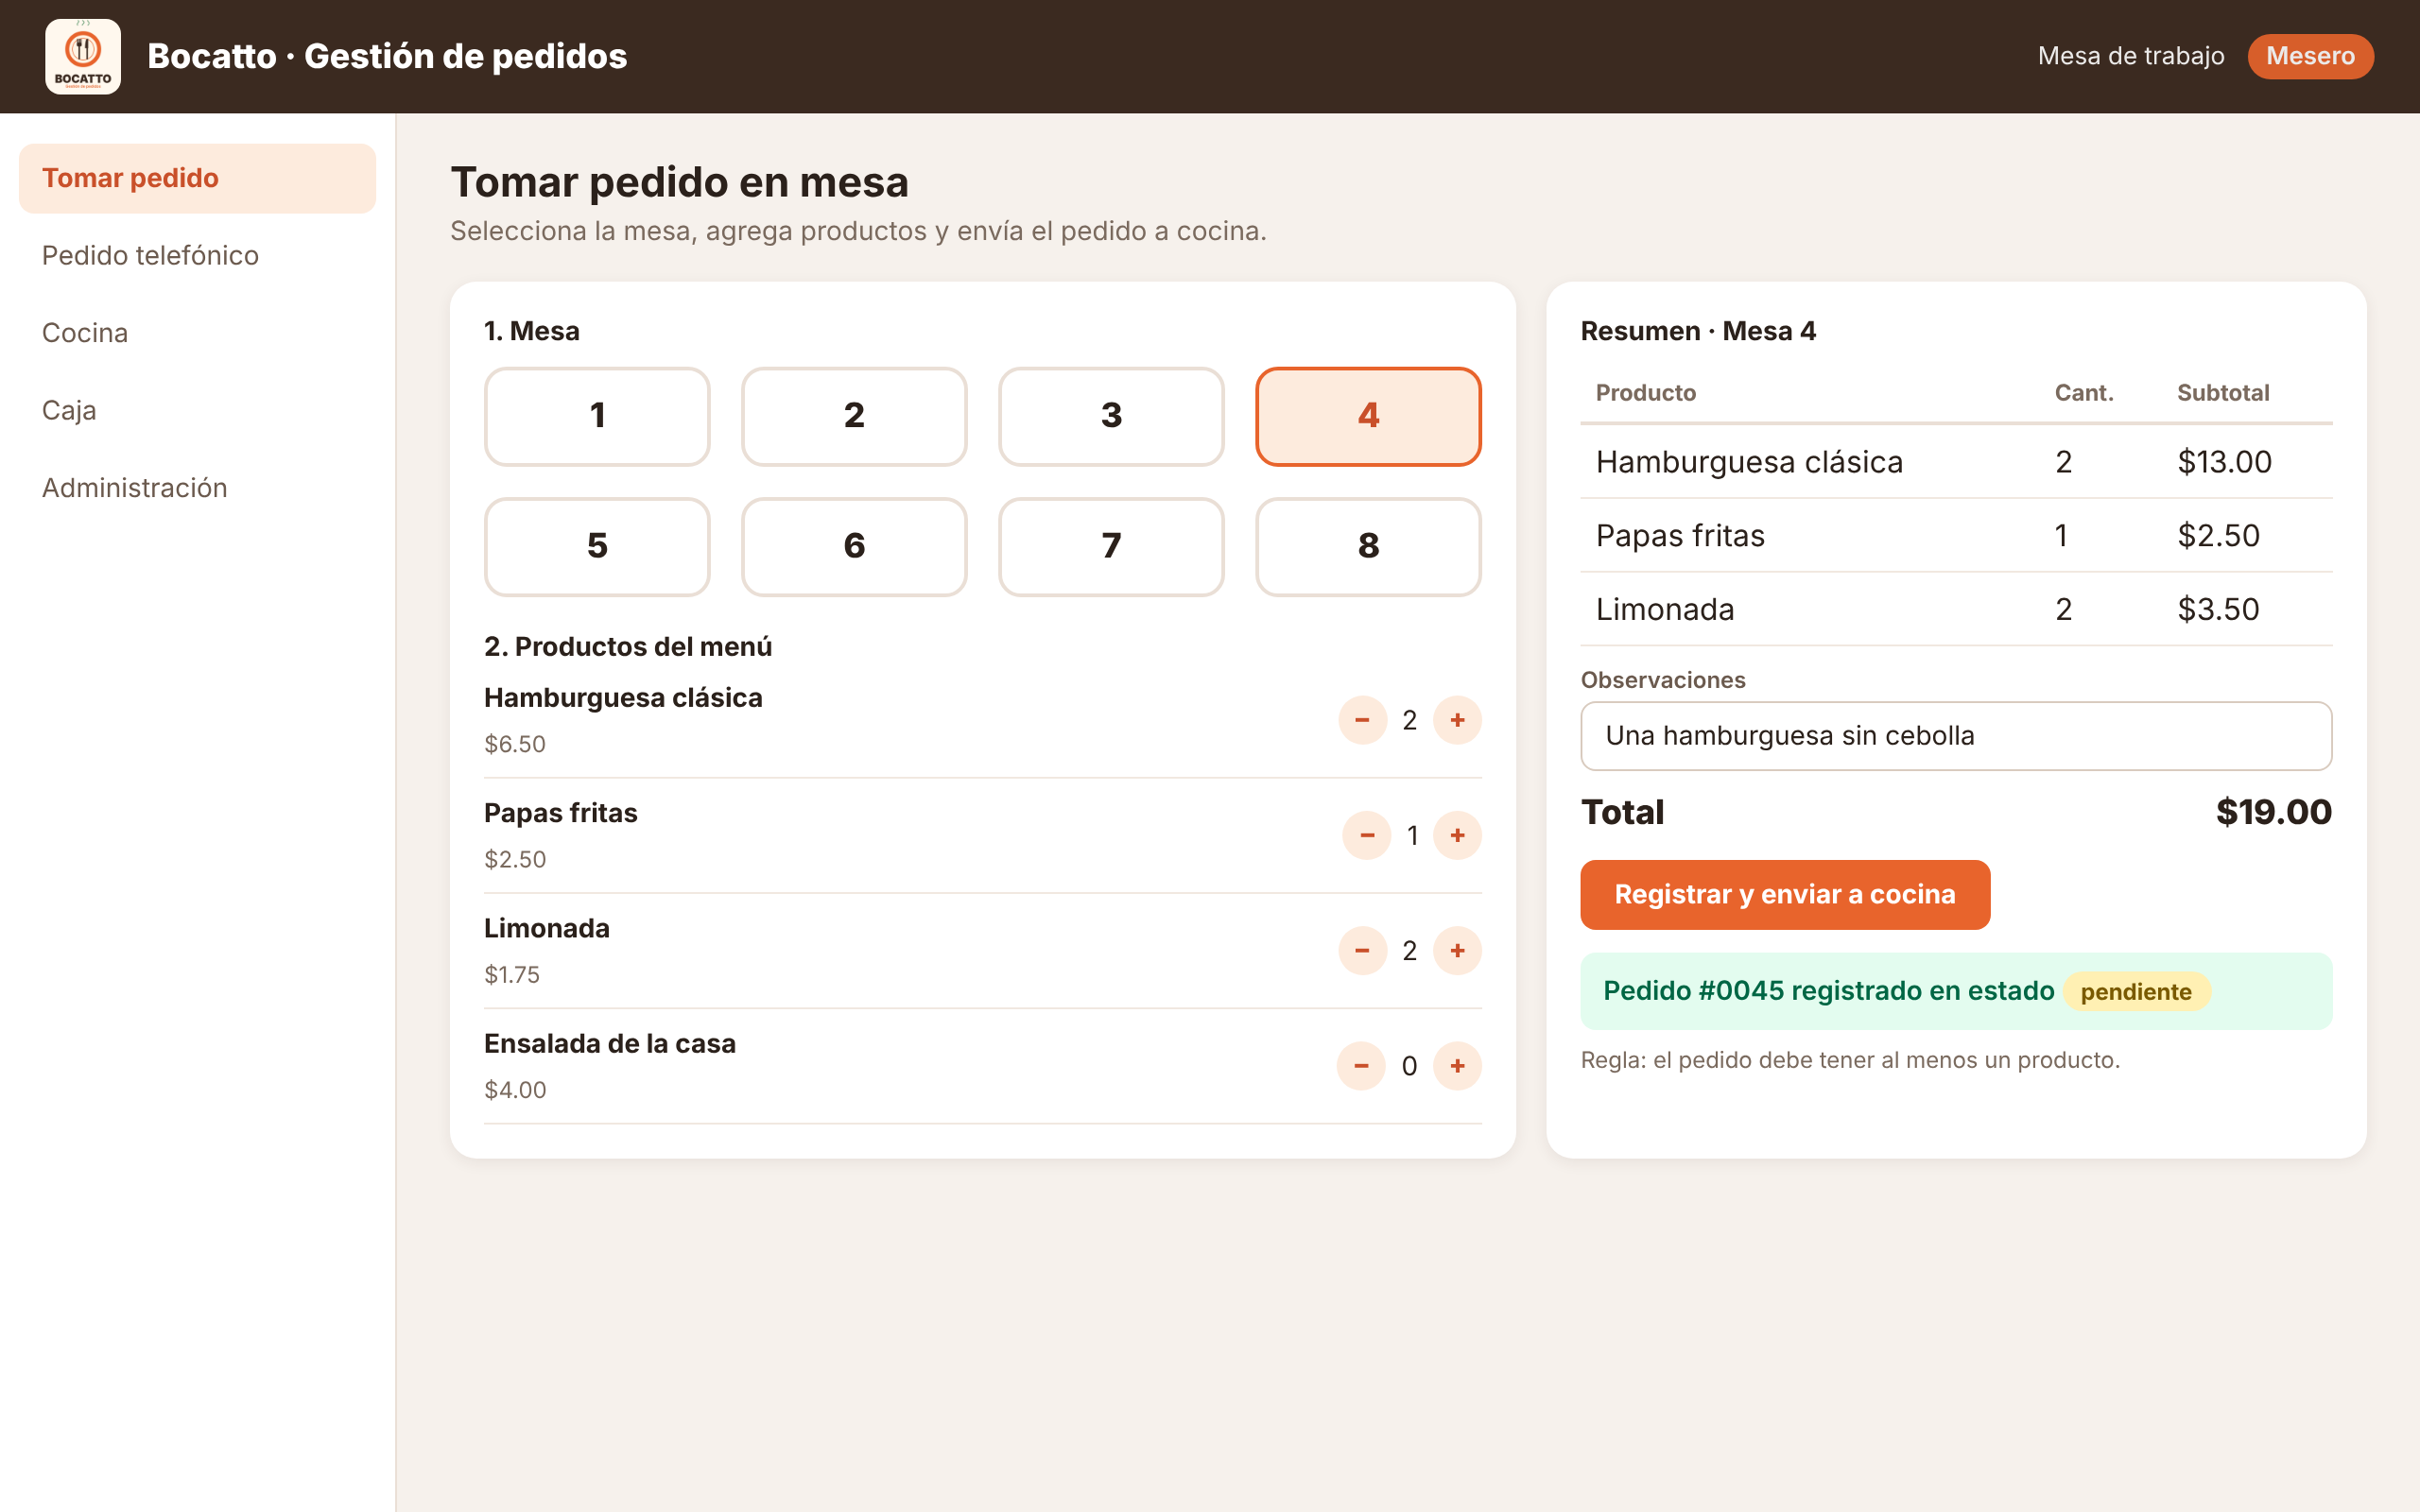
\includegraphics[width=0.85\textwidth]{RF002_pedido_mesa.png}
  \caption{Mockup de la pantalla de toma de pedido en mesa (RF002).}
  \label{fig:mock}
\end{figure}

El modelo de datos propuesto (Figura \ref{fig:modelo}) reúne las entidades que aparecen en los ocho requisitos: usuario, mesa, producto, promoción, pedido y detalle del pedido. Un pedido puede o no tener mesa, porque los pedidos telefónicos no la usan.

\begin{figure}[H]
  \centering
  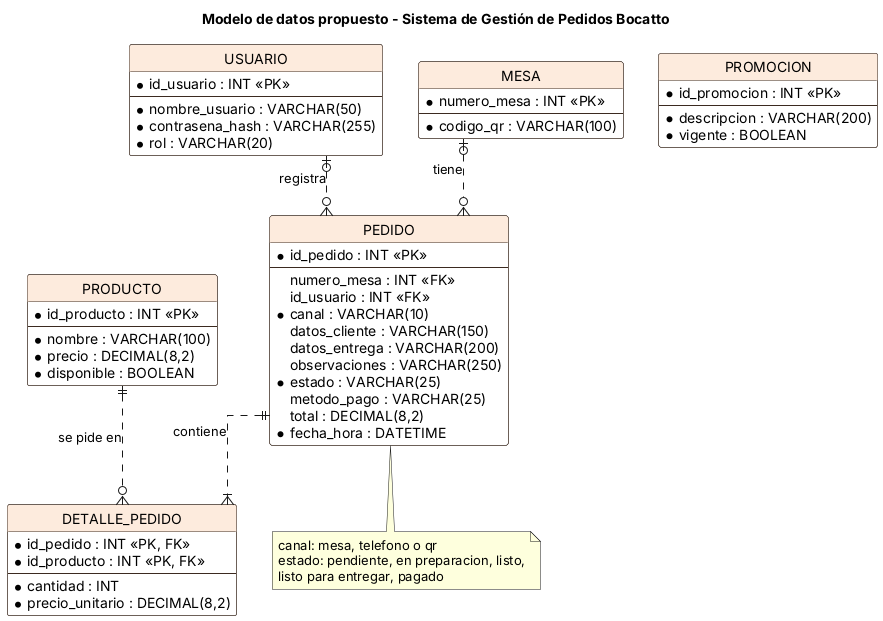
\includegraphics[width=0.85\textwidth]{modelo_datos.png}
  \caption{Modelo de datos propuesto para el sistema Bocatto.}
  \label{fig:modelo}
\end{figure}

\subsection{Reorganización del repositorio en GitHub}

El repositorio se ordenó con la estructura pedida en el taller. Las carpetas \texttt{2. DISEÑOS} y \texttt{3. CODIGO} solo tienen lo que ya existe del proyecto: los diagramas de casos de uso, las clases de análisis, las secuencias, los mockups y las piezas visuales. La carpeta de código queda lista para la siguiente unidad.

\begin{lstlisting}[language=bash]
# Estructura del repositorio RicardoLainez36838_G5_ADSW
1. ELICITACION/
   1.0 Especificación RS/
   1.1 Cronograma/
   1.2 Matriz IREB/
   1.3 Historias de usuario/
   1.4 Actas de Reunion/
   1.5 Backlog/
   1.6 Pruebas Unitarias/
   1.7 Reporte de errores/
2. DISEÑOS/
   2.1 Casos de uso nivel 0/
   2.2 Clases de analisis y secuencias/
   2.3 Mockups/
   2.4 Piezas visuales/
3. CODIGO/
ANALISIS/
DT/
Informe final/
KANBAN/
README.md
\end{lstlisting}

\begin{figure}[H]
  \centering
  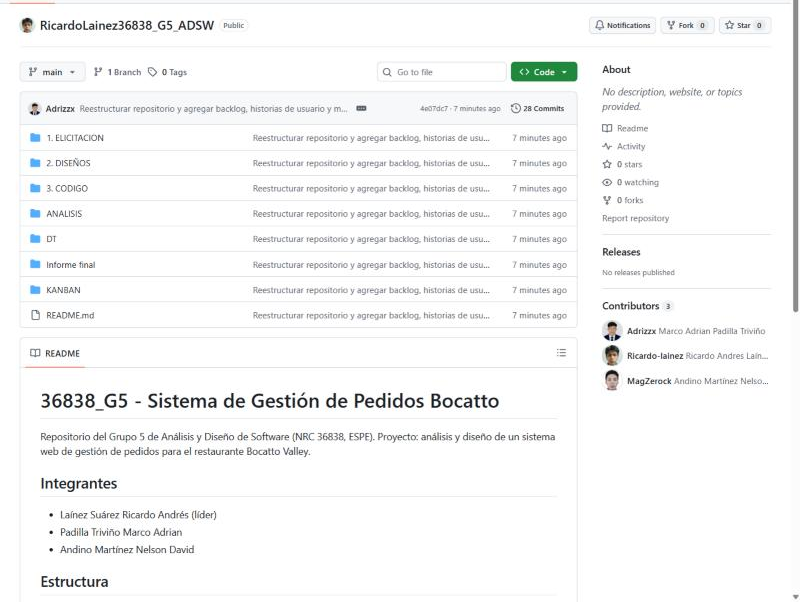
\includegraphics[width=0.9\textwidth]{github_repo.png}
  \caption{Vista del repositorio en GitHub con la nueva estructura de carpetas.}
  \label{fig:github}
\end{figure}

\subsection{Integración con el P.A.R.A. en Notion}

En la página P.A.R.A. del proyecto se agregó la sección \textit{SPRINTS - JIRA}. Tiene los enlaces al tablero, al backlog y a Confluence, y un desplegable por sprint con sus historias de Jira. La base de datos de sprints de Notion se actualizó con las actividades de esta semana y las evidencias apuntan a las nuevas rutas del repositorio.

\begin{figure}[H]
  \centering
  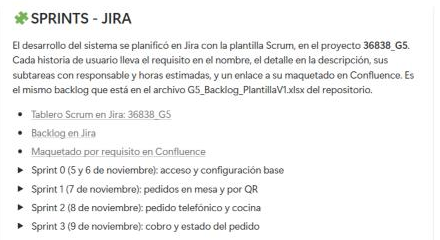
\includegraphics[width=0.8\textwidth]{notion_sprints.png}
  \caption{Sección SPRINTS - JIRA en la página P.A.R.A. del proyecto en Notion.}
  \label{fig:notion}
\end{figure}

\section{Resultados}

Se cumplió con todo lo planificado. El backlog tiene 8 historias y 26 tareas que suman 45 horas. Los cuatro sprints están registrados en Jira y lo que muestra el tablero coincide con la plantilla de Excel. Cada requisito tiene su página en Confluence enlazada a Jira. Los enlaces del proyecto son:

\begin{table}[H]
\centering
\small
\begin{tabular}{|p{3cm}|p{10.6cm}|}
\hline
\textbf{Herramienta} & \textbf{Enlace} \\ \hline
Jira (tablero) & \url{https://36838-g5.atlassian.net/jira/software/projects/SCRUM/boards/1} \\ \hline
Confluence & \url{https://36838-g5.atlassian.net/wiki/spaces/3/pages/327682} \\ \hline
GitHub & \url{https://github.com/Ricardo-lainez/RicardoLainez36838_G5_ADSW} \\ \hline
Notion (P.A.R.A.) & \url{https://www.notion.so/3f3cd8194c458048b3adf5c09e2195b6} \\ \hline
\end{tabular}
\caption{Enlaces a las herramientas del proyecto.}
\label{tab:links}
\end{table}

\section{Conclusiones}

\begin{itemize}
  \item Escribir cada requisito como historia de usuario obligó a pensar en quién usa la función y para qué. Eso ayudó a separar bien las tareas y a darles una estimación.
  \item Con sprints cortos y ordenados según el recorrido del pedido, cada entrega se apoya en lo que ya está hecho: sin acceso no hay pedidos y sin pedidos no hay cocina ni caja.
  \item Tener la misma información en la plantilla, en Jira y en Confluence permite rastrear cualquier requisito desde la ERS hasta su pantalla y su responsable.
  \item Al enlazar Jira, Confluence y GitHub con Notion, el P.A.R.A. pasó a ser el punto de entrada de todo el proyecto.
\end{itemize}

\section{Recomendaciones}

\begin{itemize}
  \item Revisar el backlog al final de cada sprint y ajustar las estimaciones con las horas reales.
  \item Usar la carpeta de pruebas unitarias y el reporte de errores del repositorio cuando empiece la implementación.
  \item Mantener los mockups de Confluence al día si cambian los requisitos, para que no se separen de la ERS.
\end{itemize}

\begin{thebibliography}{9}
\bibitem{scrumguide} K. Schwaber y J. Sutherland, \textit{La Guía de Scrum}, 2020. Disponible en: \url{https://scrumguides.org}
\bibitem{jira} Atlassian, \textit{Jira Software Cloud documentation}. Disponible en: \url{https://support.atlassian.com/jira-software-cloud/}
\bibitem{confluence} Atlassian, \textit{Confluence Cloud documentation}. Disponible en: \url{https://support.atlassian.com/confluence-cloud/}
\end{thebibliography}

\end{document}
